\documentclass[12pt]{article} 
% If you really can't fit your answers within the space provided, you could try 11pt above


\usepackage[top=1.5cm, bottom=1.5cm, left=1.5cm, right=1.5cm]{geometry}
\usepackage{color,graphicx,amsmath,mathtools,amssymb}

\newtheorem{theorem}{Theorem}[section]
\newtheorem{lemma}[theorem]{Lemma}
\pagestyle{plain}

\begin{document}  
\pagestyle{empty}
Homework 1: Nico Boyle, Owen Moorhus,  Asher Olgeirson

\noindent {\small This document is property of Northeastern University.  Unauthorized distribution of the content is not~permitted.\\}

\begin{enumerate}





\item
\begin{enumerate}
\item What set is the union of  $\{8,16, 22\}$ and the intersection of  $\{4,5,6,14,15,16,24,25,26\}$ and  $\{32,24,16,8\}$?\\\\
% Increase or decrease the number of  \\  to adjust space vertical space.  
% Alternatively you can use the \vskip command,  for instance \vskip0.2cm


{\color{blue}
Answer: \\ 
$ 
 \{8,16,22\} \cup \left(\{4,5,6,14,15,16,24,25,26\} \cap \{32,24,16,8\}\right) \\
= \{8,16,22\} \cup \{16,24\} \\
= \boxed{\{8,16,22,24\}}
$
} 



\item What set is the intersection of  $\{10, 30, 20\}$ and the union of  $\{10, 20\}$ and  $\{20, 40\}$?\\\\\\\\

  {\color{blue}
  $\{10,30,20\}\cap \left(\{10,20\}\cup\{20,40\}\right)\\
  = \{10,30,20 \} \cap \{10,20,40\} \\
  = \boxed{\{10,20 \}}
  $
  }

\item What is $\{3,5,7,9\} - \{7,6,5,4\}$?\\\\
 
  {\color{blue}
$
\boxed{\{3,9\}}
$
}

\item What is $\{4,6,5,7\} - \{3,5,7,9\}$?\\\\
  {\color{blue}
$
\boxed{\{ 4,6 \}}
$
  }

\item Let $A = \{100, 200, 4, 2, -8\}$.   Let $B= \{0, 4, -8, 100, 200\}$.  \\
What is $(A-B) - (B-A)$? \\\\
{\color{blue}
$
(A-B)=\{2\}\\
(B-A)=\{0\}\\
\{2\}-\{0\} = \boxed{\{2\}}
$
  }

\item Let $A = \{100, 200, 4, 2, -8\}$.   Let $B= \{0, 4, -8, 100, 200\}$\\
What is  $A - (A - B)$? \\\\

{\color{blue}
$
(A-B)=\{2\}\\
A-\{2\}=\boxed{ \{ 100,200,4,-8 \} }
$
}
\item
Use set builder notation to express $\{3,7,11,15,\ldots , 403\}$, as compactly as possible, with as little English as possible. \\
{\color{blue}
  Assuming $0\in {\Bbb N}$ \\
$
% \{ x \in \mathbb{Z} |3\leqslant x+4 \leqslant 403 \}
\boxed{\{x\in {\Bbb N}|3+4x\leqslant 403\}}
$
}

\end{enumerate}



%%%%%%%%%%%%%%%%%%%%%%%%%%%%%%%%%%%%%%%%%%%%%%%%
\newpage

\noindent {\small Property of Northeastern University.  Unauthorized distribution of the content is not~permitted.}



\item 
Consider the following sets: 
$H = \{$herbivores$\}$.           			
$S=\{$animals with sharp teeth$\}$.      	
$R = \{$animals that run fast$\}$.              
$L=\{$animals with long necks$\}$.             

\begin{enumerate}


\item
Use set notation (e.g., union, intersection, etc) to describe herbivores that have sharp teeth or run fast.  
Your expression should be as simple as possible. 
{\em  Do not use set  builder notation.}\\\\
{\color{blue}
  $
  \boxed{H\cap (S \cup R)}
  $
}


\item
To survive the next ice age, members of a species must have sharp teeth  or   run fast,  but they  must   also have long necks  or have sharp teeth.
Express these conditions using set notation, minimizing redundancy. \\\\
%{\em  (Not set builder notation)}\\\\\\
{\color{blue}
$
\boxed{S\cup (L \cap R)}
$
}


\item
In a certain herbivore ecosystem,  there are 52 species that have sharp teeth or can run fast. 
18 of these species have both qualities.  25 species have sharp teeth.  
How many of the 52 species can run fast? (Briefly show how you calculated this, and name the most relevant  concept in the calculation) \\
{\em It is ok to use the symbol of a set to denote its size, if context is clear; no need to use $|$ $|$.} \\
{\color{blue}

  Based on the inclusion-exclusion principle that states $S+R=(S\cup R)+(S\cap R)\\\\$
$
R=(S\cup R) + (S\cap R) - S \\
= 52 + 18 -25 \\
=\boxed{R = 45}
$\\
(Help recived from Rahul Rao)
}


\item
The ecosystem mentioned in (c)  contains  100 species.
\begin{enumerate}
\item
How many don't have sharp teeth and can't run fast?  Use  deMorgan's laws.\\\\
{\color{blue} deMorgan's Laws state: $$\overline{A\cup B} = \overline{A} \cap \overline{B}$$\\
  $
  \therefore \overline{S \cup R} = \overline{S} \cap \overline {R} = 48
  $
}

\item
How many  don't have sharp teeth or can't run fast (or both)?  Use deMorgan.\\\\

{\color {blue}
  deMorgan's laws state: $\overline{S\cup R} = \overline{S}\cap \overline{R}$ \\
  $\therefore \overline {S} \cap \overline {R} = 100-52=48$
}
\end{enumerate}


\end{enumerate}







%%%%%%%%%%%%%%%%%%%%%%%%%%%%%%%%%%%%%%%%%%%%%%%%
\newpage
\noindent {\small Property of Northeastern University.  Unauthorized distribution of the content is not~permitted.\\}



\item 100 people participated in a brief poll.   Everyone answered either yes or no to each question. The first question was ``Do you like cookies?", to which 45 answered yes. The second question was ``Do you like milk?", to which 21 answered yes.  You observe that 15 people liked both cookies and milk. 
Draw a Venn diagram that represents the sets of people who like cookies, and those who like milk (among those who took the poll). Place numbers in your figure so that everyone is represented.  Each disjoint ``section" of the diagram should have a number that corresponds only to that section. By definition ``sections" do not overlap.  \

\begin{center}
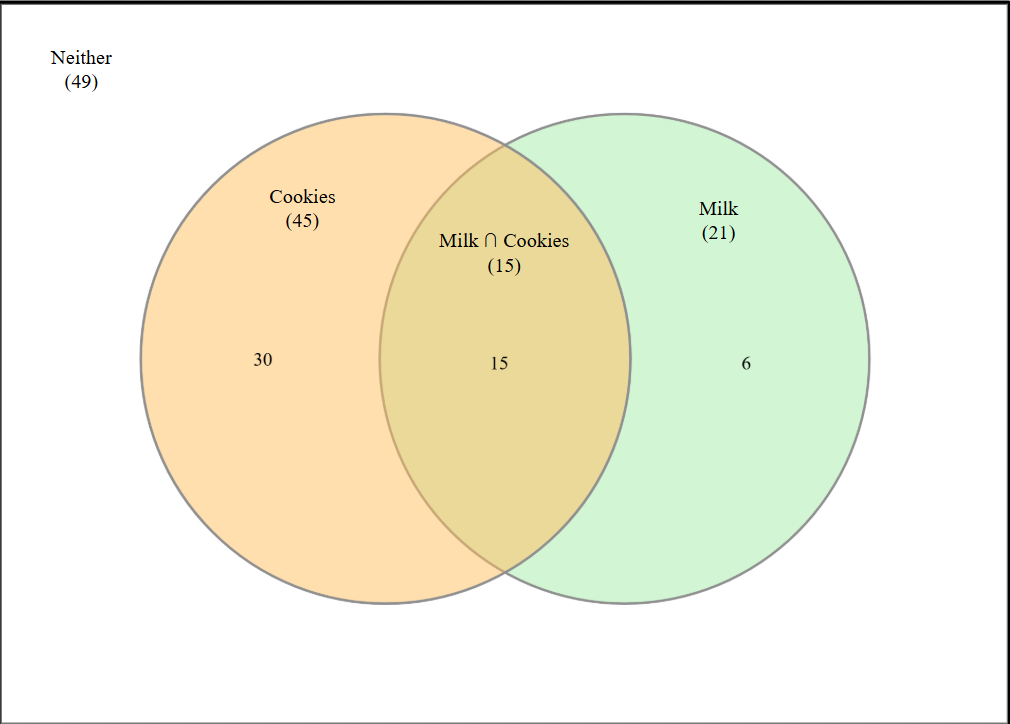
\includegraphics[width=5.5in]{Venn.png}   
\end{center}
% Adjust width as needed.  Change file name and type as needed.




\item
Let $f(n) = n^2 -10n + 27$.   Prove that $f(9) < f(11)$.  This must be done by writing the expression for  $f(9)$ on the first line, then on each new line starting with the symbol for equality or inequality, and making one algebraic step.  The last line should conclude with $f(11)$, so that when we read all of the lines together we see a chain of equalities or inequalities, such that the first and last expression show what we want to prove.  This exercise is more about proof style than algebra.  You should aim for simplicity, efficiency, and clarity.  \\

{\color{blue}
\em{Proof: $f(9)<f(11)$}\\
$
Let\ f(n):=n^2-10n+27 \ \text{where n is a real number}\\
f(9)=9^2-10(9)+27=18 \\
< (9+2)^2 -10(9+2)+27 \\
< 38 = f(11) \\
\therefore f(9)=18<f(11)=38\\
\blacksquare
$
}






%%%%%%%%%%%%%%%%%%%%%%%%%%%%%%%%%%%%%%%%%%%%%%%%
\newpage
\noindent {\small Property of Northeastern University.  Unauthorized distribution of the content is not~permitted.\\}

\item
Suppose that we play a variant of {\em Chomp} on a hexagonal board like the one below. The poisoned cookie is marked as {\bf P}.
Whenever you take a cookie, you must also take everything within its ``upper-right" $120^{\circ}$ cone. For example, if you take the middle cookie in the illustration then you must take cookies 1 through 9 and everything else in the marked region.

\begin{center}
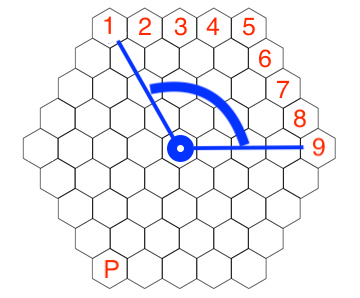
\includegraphics[width=1.9in]{grid.png}
\end{center}



Prove that Player 1 can win this game, with a non-constructive proof. \\

{\color{blue}
1. Suppose player 1 eats the upper rightmost cookie marked 5 on the figure above.\\
2. This leaves player 2 with a board that, given all possible moves by player 2, could have been made by player 1 on the first move. \\
3. Zermello's theorem states that in any game of perfect information, one of the two players has a winning strategy.  \\
4. Since player 2 cannot have a winning strategy (because player 1 could have made the first move that player 2 made), player 1 must have a winning strategy.\\ 
} 







\end{enumerate} 




\end{document}

